\documentclass{article}
\usepackage[utf8]{inputenc}
\usepackage[spanish]{babel}
\usepackage{graphicx}
\usepackage{float}
\usepackage{adjustbox}
\usepackage{fancyhdr}
\usepackage[compact]{titlesec}        
\usepackage{geometry}

\geometry{
    a4paper,
    total={170mm,257mm},
    left=40mm,
    right=40mm,
    top=35mm,
    bottom=35mm,
}

\pagestyle{fancy}
\fancyhf{}
\lhead{KeyPaX, Bárbaros Software S.A.}
\rhead{\thepage}
\lfoot{Propuesta técnica y económica}
\renewcommand{\footrulewidth}{0.4pt}

\setlength{\parindent}{2em}
\setlength{\parskip}{1em}

\title{
\Huge{KeyPaX, Bárbaros Software S.A.} \\ 
\begin{Large} 
Propuesta técnica y económica del proyecto
\end{Large}}
\author{}
\date{22 de febrero de 2021}

\begin{document}

\maketitle

\pagebreak

\section{Resumen Ejecutivo}

En el siguiente documento se presenta el sistema KeyPaX, va a ser desarrollado por Bárbaros Software S.A. y permite gestionar contraseñas almacenadas remotamente en los servidores del sistema. Permite almacenar junto con las contraseñas el nombre de usuario, URL y la fecha de creación, entre otros. Las contraseñas se pueden organizar por categorías y los usuarios pueden realizar búsquedas entre sus contraseñas en base a ciertos parámetros.

Además, para mejorar la seguridad del sistema, se podrán generar automáticamente contraseñas robustas con longitud y caracteres variables. El usuario accederá al servicio mediante una contraseña maestra y deberá identificarse por primera vez para cada dispositivo con 2FA.

Para acceder al sistema se utilizará la aplicación para móviles Android o en diferentes navegadores web. Se utilizará Java (Android SDK) y JavaScript (React.JS), respectivamente, para implementar las vistas del sistema. El \textit{backend} se desarrollará utilizando Node.JS y la librería Express. Por último, la base de datos utilizará el gestor de base de datos MongoDB. 

El despliegue del sistema se realizará en un entorno de contenedores Docker. Mediante Docker se puede aprovechar al máximo los recursos \textit{hardware} de la máquina, aumentando la portabilidad del sistema y ahorrando en fallos del desarrollo. 




\pagebreak

\tableofcontents

\pagebreak

\section{Objetivos del sistema}

% Descripción breve de las necesidades que el sistema debe abordar y la funcionalidad que se desarrollará para para cubrir estas necesidades.

KeyPaX permite gestionar una colección de contraseñas de manera segura y remota. Permite almacenar los nombres de usuario y claves de acceso a distintos servicios, además de otra información adicional como URL y fechas de creación y actualización. Estas contraseñas se pueden organizar por categoría y realizar búsquedas según sus campos. El sistema puede generar contraseñas robustas y configurables por el usuario. El usuario accederá a su colección de contraseñas mediante una contraseña maestra y realizará 2FA en las ocasiones requeridas. Se accederá al sistema mediante una interfaz web o una aplicación móvil.

\subsection{Análisis de requisitos preliminar}

\begin{table}[H]
    \centering
    \begin{tabular}{| c | p{30em} |}
    \hline
        Código &  Descripción  \\ \hline
        RF-1 & El sistema permite almacenar contraseñas \\ \hline
        RF-1.1 & El sistema permite almacenar pares que constan de nombre de usuario y contraseña  \\ \hline
        RF-1.2 & El sistema permite asociar a las contraseñas una URL del sitio web al que corresponden \\ \hline
        RF-1.3 & El sistema registra la fecha de creación y actualización de la contraseña \\ \hline
        RF-1.4 & El sistema permite almacenar una descripción de texto. \\ \hline
        RF-2 & El  sistema permite organizar las contraseñas por categorías \\ \hline
        RF-3 & El sistema permite realizar una búsqueda entre las contraseñas por categoría, fecha de creación y actualización  \\ \hline
        RF-4 & El sistema permite generación de contraseñas pseudoaleatorias \\ \hline
        RF-4.1 & El sistema permite seleccionar la longitud de la contraseña a generar\\ \hline
        RF-4.2 & El sistema permite seleccionar el conjunto de caracteres que compone la contraseña a generar\\ \hline
        RF-4.3 & El sistema mostrará el grado de robustez de la contraseña al ser generada \\ \hline
        RF-5 & El sistema permite al usuario acceder a sus contraseñas únicamente a través de la contraseña maestra \\ \hline
        RF-6 & El sistema requiere 2FA para iniciar sesión desde un dispositivo nuevo, distinto a los utilizados con anterioridad \\ \hline
        RF-7 & El usuario se registra en el sistema mediante un correo electrónico y una contraseña maestra\\ \hline
        RF-7.1 & El registro de sesión se deberá confirmar, para verificar la identidad, mediante un correo al usuario registrado \\ \hline
        RF-8 & El sistema permite la actualización de las contraseñas. \\ \hline
        RF-9 & Se accede al sistema mediante una aplicación móvil \\ \hline
        RF-10 & Se accede al sistema mediante una interfaz web \\ \hline
    \end{tabular}
\end{table}

\pagebreak

\section{Descripción técnica}

\subsection{Aspectos técnicos de relevancia para los usuarios}

El acceso al repositorio de contraseñas de KeyPaX requiere de conexión a internet. Las contraseñas no son guardadas en el dispositivo del usuario para evitar desajustes de versionado y limitar la posibilidad de pérdida/\textit{leaking} de las contraseñas.

El sistema KeyPaX permite a los usuarios acceder al repositorio mediante dos interfaces:
\begin{itemize}
    \setlength\itemsep{0em}
    \item Navegador web. El sistema funcionará al 100\% de sus capacidades en los siguientes navegadores web: Google Chrome, Firefox, Safari. En el resto de navegadores, el sistema puede no cargar ciertos componentes.
    \item Aplicación Android. La versión del sistema debe ser al menos 6.0 "Marshmellow".
\end{itemize}

\subsection{Aspectos técnicos de relevancia para los clientes}

El sistema está diseñado para ser desplegado en un entorno de contenedores Docker.
Se ha escogido esta tecnología de despliegue por su alto aprovechamiento de los recursos de la máquina host y portabilidad a través de distintas máquinas.
Dicho esto, a término del plazo de desarrollo del producto, el sistema quedará desplegado en un clúster remoto accesible vía internet por los usuarios. Dicho clúster remoto será de propiedad ajena a la empresa y los clientes deberán acarrear con los costes de mantenimiento y alquiler de las máquinas que imponga el proveedor de \textit(cloud).
Sin embargo, el código fuente completo del producto junto con manuales de despliegue serán entregados a los clientes, por tanto, estos puede decidir migrar el despliegue del sistema a máquinas propias que cumplan con los requisitos establecidos en los manuales.

\pagebreak

\subsubsection*{Tecnologías}

Se utilizaran las siguientes tecnologías para cada una de las capas:

\begin{itemize}
    \setlength\itemsep{0em}
    \item \textit{Frontend} (Móvil Android): Java, Android SDK
    \item \textit{Frontend} (Navegador Web): JavaScript, React.JS
    \item \textit{Backend}: Node.JS, Express
    \item Base de datos: MongoDB
\end{itemize}

\subsubsection*{Despliegue}

El producto será desplegado en distintos componentes dockerizados:

\begin{itemize}
    \setlength\itemsep{0em}
    \item \textit{Frontend}: Constituye la interfaz de usuario. Se separa en dos componentes, \textit{frontend} para la aplicación móvil y \textit{frontend} para la interfaz web.
    \item \textit{Backend}: Constituye el cerebro del sistema, se encargará de atender todos los aspectos necesarios para que el sistema desarrolle el comportamiento diseñado.
    \item Base de datos: Almacenará la información de los usuarios y aquella necesaria para el funcionamiento del sistema.
\end{itemize}

\begin{figure}[H]
    \centering
    \begin{adjustbox}{max size={\textwidth}{\textheight}}
        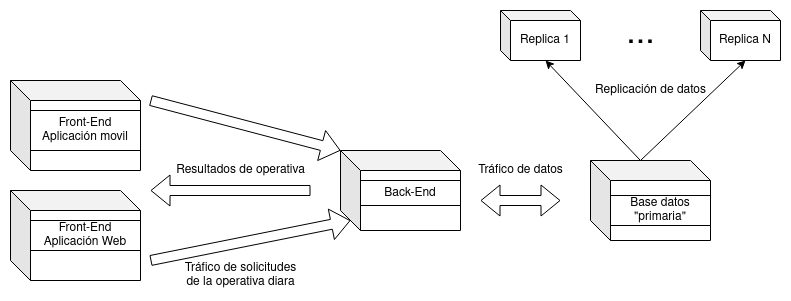
\includegraphics{../images/desplieguev1.png}
    \end{adjustbox}
    \caption{Primera versión del diagrama de despliegue}
    \label{despliegueV1}
\end{figure}

\subsubsection*{Análisis de riesgos y planes de contingencia}

El mayor riego en el que incurre el sistema es la exposición de los datos de los usuarios a causa de una ataque a la base de datos. 
Para reducir el impacto y ocurrencia de este posible evento se propone limitar el acceso al componente de base de datos mediante contraseñas robustas, autentificación del origen de las peticiones a la base de dato y cifrado de la información.

Para prevenir ataques de tipo \textit{ransomware} o el borrado malicioso de la información, se replicará la información de la base de datos a lo largo de un conjunto de replicas, lo cual permite disponer de un \textit{back-up} de los datos para permitir el funcionamiento del sistema si ocurriese alguno de estos eventos.

En cuanto ataques contra la disponibilidad del sistema, se implementarán los cortafuegos necesarios para asegurar la disponibilidad en todo momento.


\pagebreak


\section{Plan de trabajo}
A continuación se va a presentar un primer boceto de plan de trabajo con fechas importantes para los clientes.

\begin{table}[H]
    \centering
    \begin{tabular}{| c | p{30em} |}
    \hline
        Fecha &  Descripción  \\ \hline
        22/02/2021 & Presentación de la propuesta técnica y económica.  \\ \hline
        02/03/2021 & Reunión de \textit{feedback} con los clientes para aprobación/negociación de la propuesta técnica y económica anteriormente presentada. Comienzo de la redacción del plan de gestión, análisis y diseño. \\ \hline
        15/03/2021 & Presentación de la primera versión del plan de proyecto.\\ \hline
        22/03/2021 & Reunión de seguimiento con los clientes. \\ \hline
        14/04/2021 & Presentación de la segunda versión del plan de proyecto. \\ \hline
        15/04/2021 & Demostración a los clientes de la primera versión desplegada.
        Entrega de documentación generada hasta el momento y transferencia del código de la versión primera del sistema.\\ \hline
        03/05/2021 & Segunda reunión de seguimiento con los clientes. \\ \hline
        21/05/2021 & Demostración a los clientes de la segunda versión desplegada.
        Entrega de documentación generada hasta el momento y transferencia del código de la versión segunda del sistema.\\ \hline
        01/06/2021 & Entrega final del producto. Consistirá en la entrega del código fuente final, manuales de usuario en formato video y texto y delegación de control del producto ya instalado en servidores de acceso públicos.\\ \hline
    \end{tabular}
\end{table}

\pagebreak

\section{Equipo técnico encargado del proyecto}

\textbf{Bárbaros Software S.A.} cuenta con tres años de permanencia en el mercado, que han proporcionado una amplia experiencia en el mundo empresarial y nos avala como una empresa referente en el sector. La empresa se caracteriza por tener una filosofía basada en el trabajo coordinado en grupo, con especialistas en distintos campos del sector que unificados forman un equipo de trabajo altamente sofisticado.
Los servicios y capacidades que nuestros clientes han podido destacar entre los más importantes son:
\begin{itemize}
    \setlength\itemsep{0em}
    \item Experiencia en desarrollo móvil en dispositivos Android.
    \item Veteranía en el \textit{framework} de JavaScript React para Web y Móvil.
    \item Destreza en el entorno de ejecución NodeJS con el \textit{framework} Express.
    \item Práctica en Bases de Datos relacionales (Oracle, Postgresql, MySql...).
    \item Conocimiento en Base de Datos no relacionales (MongoDB).
    \item Alta uso de diferentes lenguajes de programación (Java, JavaScript, C, C++, GoLang).
    \item Estudio de metodología de despliegue de Proyectos con Docker y Kubernetes.
    \item Maestría en el uso de \textit{IaaS} (Microsoft Azure, Amazon AWS).
    \item Prácticas de \textit{testing} con PostMan.
    \item Altos conocimientos en gestión de versiones a través del Software Git.
\end{itemize}

Bárbaros Software S.A. proviene de la famosa Barbara Liskov, científica de la computación estadounidense reconocida con la medalla John von Neumann (2004) y el premio Turing (2008).

La empresa ha participado en projectos similares, realizando un sistema de gestión de notas en dispositivos móviles, por ejemplo. Además, se ha participado en varias hackatones, entre ellas, la Adidas uCode, celebrada en la EINA. 


\pagebreak

\subsection*{Integrantes del equipo}

En cuanto a las características individuales de los 6 integrantes de la empresa:
\begin{itemize}
   \item Arturo Calvera Tonin, actualmente colaborando con el departamento de investigación de la EINA y el I3a en el desarrollo de un sistema de control de acceso a aulas dentro de la universidad. Notable experiencia en sistemas distribuidos y en varios sistemas de información donde poder gestionar todos los datos de nuestro producto.
   \item Jorge Bernal Romero, gran capacidad de polivalencia en los aspectos generales del proyecto. Altamente implicado en su comunidad local participando frecuentemente en programas de voluntariado. Destacar participación en relaciones internacionales y conocedor del comercio electrónico.
   \item Andoni Salcedo Navarro, consta un amplio conocimiento y experiencia en la programación con distintos lenguajes en una amplia variedad de ámbitos. Domina un gran número de tecnologías de almacenamiento y gestión de datos así como los lenguajes con los que se gestionan.
   \item Javier Vela Tambo, en vistas a trabajar el año que viene en el extranjero, concretamente en la universidad de Rhode Island, en busca de continuar con su formación y ampliar sus conocimientos.
   \item JJorge Borque Benedí, familiarizado con una gran variedad de medios y dispositivos gracias a las distintas experiencias que ha obtenido trabajando con estos a lo largo de su trayectoria. Gran profesional en medidas de seguridad.
   \item Carlos Bellvis Irache, disfruta de una alta capacidad de liderazgo, motivación de grupo y resolución de conflictos. Todo ello debido a su trabajo actual como entrenador de un equipo de fútbol, dónde aprende a lidiar con derrotas prácticamente semanalmente.
\end{itemize}


Estas características individuales permiten afrontar los problemas mediante distintos puntos de vista y con ello conseguir cohesionar en los productos finales un resultado satisfactorio para los clientes.

\pagebreak

\section{Presupuesto}

Nombre apellidos, domiciliada para estos efectos en Zaragoza, provincia de Zaragoza calle , y DNI número DNI, en nombre y representación de Bárbaros Software S.A. con C.I.F. y domicilio fiscal en Zaragoza, calle María de Luna número 3, enterada del anuncio publicado en el "B.O.E." del día 12 de febrero de 2021 y de las condiciones y requisitos que se exigen para la adjudicación de los servicios de KeyPaX, provincia de Zaragoza, se compromete a tomar a su cargo la ejecución de los mismos, con estricta sujeción a los requisitos y condiciones expresados, por las cantidades que se encuentran en concepto de precio, indicándose igualmente el IVA a soportar por la Administración, en cada caso, según las soluciones siguientes:


\begin{table}[H]
    \centering
    \begin{tabular}{| c | c | p{15em} |}
    \hline
        SOLUCIÓN &  CANTIDAD EUROS & CANTIDAD LETRA \\ \hline
        BASE Precio & 19.940 & Diecenuevemil novecientos cuarenta.\\ \hline
        IVA Admón. &  4.187,4 & Cuatromil ciento ochenta y siete con cuarenta.\\ \hline
        TOTAL Precio &  24.127,4 & Veinticuatromil cientro veintisiete con cuarenta.\\ \hline
    \end{tabular}
\end{table}

El licitador hace constar que el precio o precios del contrato ofertado incluye el importe de las tasas que sean de aplicación, con conformidad con lo señalado en el Pliego de Cláusulas Administrativas Particulares que rige este contrato.

Atentamente,

\pagebreak

\section*{Anexo I. Glosario}
\addcontentsline{toc}{section}{Anexo I. Glosario}

\begin{description}
    \setlength\itemsep{0em}
    \item[2FA] \textit{Two-Factor Authentication}. Método de autentificación que requiere dos tipos de información del usuario. Normalmente una contraseña y un código enviado al correo electrónico o teléfono móvil.
    \item[API] \textit{Application Programming Interface}. Conjunto de procedimientos que ofrece cierta biblioteca o sistema para ser utilizado por otro \textit{software} e interaccionar con él abstrayendo ciertos aspectos.
    \item[Contraseña] Clave alfanumérica y que puede contener símbolos, para identificarse en un servicio o cuenta de internet. En el documento, se refiere, además, a toda la información relativa a estas (URL, descripción, fechas, ...).
    \item[Framework] Plataforma para desarrollar aplicaciones software que ofrece una estructura inicial en la que los desarrolladores pueden construir para una plataforma específica. 
    \item[IaaS] \textit{Infrastructure as a Service}. Servicios en línea, generalmente \textit{cloud}, que proporcionan APIs de alto nivel que permiten abstraer detalles de infraestructura.
    \item[URL] \textit{Uniform Resource Identifier}. En este contexto, la dirección de la página web. 
\end{description}

\section*{Anexo II. Estimación de costes}
\addcontentsline{toc}{section}{Anexo II. Estimación de costes}

%\section*{Anexo III+. Otros anexos}
%\addcontentsline{toc}{section}{Anexo III+. Otros anexos}

\end{document}  